%%%%%%%%%%%%%%%%%%%%%%%%%%%%%%%%%%%%%%%%%
% Uppsala University Assignment Title Page 
% LaTeX Template
% Version 1.0 (27/12/12)
%
% This template has been downloaded from:
% http://www.LaTeXTemplates.com
%
% Original author:
% WikiBooks (http://en.wikibooks.org/wiki/LaTeX/Title_Creation)
% Modified by Elsa Slattegard to fit Uppsala university
% License:
% CC BY-NC-SA 3.0 (http://creativecommons.org/licenses/by-nc-sa/3.0/)

%\title{Title page with logo}
%----------------------------------------------------------------------------------------
%	PACKAGES AND OTHER DOCUMENT CONFIGURATIONS
%----------------------------------------------------------------------------------------

\documentclass[12pt]{article}
\usepackage{geometry}
\geometry{a4paper,scale=0.75}
\usepackage[english]{babel}
\usepackage[utf8x]{inputenc}
\usepackage{amsmath}
\usepackage{graphicx}
\usepackage{float}
\usepackage[colorinlistoftodos]{todonotes}
\usepackage[ruled]{algorithm2e}
\usepackage{booktabs}
\usepackage{url}
\usepackage[colorlinks]{hyperref}
\usepackage{amssymb}
\usepackage{indentfirst}
\setlength{\parskip}{0.5\baselineskip}
\setlength{\parindent}{0em}
\usepackage{appendix}
\usepackage{subfigure}


\begin{document}

\begin{titlepage}

\newcommand{\HRule}{\rule{\linewidth}{0.5mm}} % Defines a new command for the horizontal lines, change thickness here

\center % Center everything on the page
 
%----------------------------------------------------------------------------------------
%	HEADING SECTIONS
%----------------------------------------------------------------------------------------

\textsc{\LARGE University of Science and Technology of China}\\[1.5cm] % Name of your university/college

\includegraphics[scale=.3]{ustc_logo_fig.pdf}\\[1cm] % Include a department/university logo - this will require the graphicx package
\textsc{\Large Introduction to Machine Learning}\\[0.5cm] % Major heading such as course name
\textsc{\large 210709}\\[0.5cm] % Minor heading such as course title

%----------------------------------------------------------------------------------------
%	TITLE SECTION
%----------------------------------------------------------------------------------------

\HRule \\[0.4cm]
{ \huge \bfseries Course Project Report}\\[0.4cm] % Title of your document
\HRule \\[1.5cm]
 
%----------------------------------------------------------------------------------------
%	AUTHOR SECTION
%----------------------------------------------------------------------------------------

\begin{minipage}{0.4\textwidth}
\begin{flushleft} 
\large\emph{Author:}\\
\large Shuxian \textsc{Bi}: PB17121707\\
Jianbai \textsc{Ye}: PB17121732\\
Xiaolong \textsc{Luo}: PB18151853\\
\end{flushleft}

\end{minipage}\\[2cm]

% If you don't want a supervisor, uncomment the two lines below and remove the section above
%\Large \emph{Author:}\\
%John \textsc{Smith}\\[3cm] % Your name

%----------------------------------------------------------------------------------------
%	DATE SECTION
%----------------------------------------------------------------------------------------

{\large \today}\\[2cm] % Date, change the \today to a set date if you want to be precise

\vfill % Fill the rest of the page with whitespace

\end{titlepage}

\tableofcontents

\newpage

\section{Introduction}
Learning to control an agent to make wise decisions in an observed environment is a unremitting pursue for researchers in Artificial Intelligence for decades.

Recent years' magnificent progress in deep learning, especially the progress in computer vision, has made it possible for agents to settle more complicated environments such as video games\cite{DBLP:journals/corr/MnihKSGAWR13}, go\cite{DBLP:journals/nature/SilverHMGSDSAPL16}, and even playing mahjong\cite{DBLP:journals/corr/abs-2003-13590}. 

In this work, we mainly focus on training a smart agent to play two Atari games: LunarLander and RiverRaid in gym environment. And our efforts are threefold.
\begin{itemize}
    \item We constructed DQN networks mainly based on \cite{DBLP:journals/nature/MnihKSRVBGRFOPB15} and obtained a quite satisfactory score.
    \item We handcrafted the backpropagation module for the Q-network as well as the RMSprop optimizer.
    \item We explored some useful tricks such as \emph{soft update} method to further improve the performance of our agent.
\end{itemize}

Our code is open source and available on Github\footnote{ \url{https://github.com/gusye1234/ML-project-2020}}.

\section{Preliminary}
\emph{Q-Learning Algorithm} \cite{watkins92a} is a classic method in Reinforcement Learning, which maintains a Q-table and takes a state and an action as input, then outputs the corresponding Q-value. Though its simplicity has made it one of the basic model in RL, when tackling with a continuous and complex environment like video games, it's neither possible to traverse all possible states nor hold a large Q table. Thus researchers are dedicated in finding a method to estimate Q values rather than store them directly.

The huge success of the applications of Deep Neural Networks in computer vision \cite{krizhevsky2012imagenet} has made it possible to estimate Q values through a neural network. In 2013, Mnih et al. \cite{DBLP:journals/corr/MnihKSGAWR13} proposed a novel framework \emph{Deep-Q-Network} which is able to train an agent and over perform most linear models in Atari games. In their model, they use a Convolution Neural Network which takes an observed states as input and then estimate the values corresponding to each possible actions. And they maintained a \emph{Reply Buffer} to settle the dynamic and correlated issue, as well as train the parameters in the Q-Network.

However, the consistent change of parameters in Q-Network has made the policy unstable, thus made it harder to train the network. Therefore, Mnih et al. \cite{DBLP:journals/nature/MnihKSRVBGRFOPB15} proposed an enhanced DQN model with a main network and a target network to address this problem, which is the main architecture we refer to in this coursework. The pseudocode of the algorithm is shown in Algorithm \ref{dql}.

\begin{algorithm}[t]
\caption{Deep Q-Learning Algorithm with Soft Update Strategy}\label{dql}
\LinesNumbered 
Initialize replay memory $\mathcal{D}$ to capacity $N$\; 
Initialize action-value function $Q$ with random weights $\theta$\; 
Initialize target action-value function $Q^{-}$ with random weights $\theta^{-}$\; 
Initialize $\epsilon, \tau \in (0, 1)$ $ (  \tau \ll 1 ) $ \; 
\For{$episode=1,2,\dots,M$}{
    \For{$t=1,2,\dots,T$}{
        With probability $\epsilon$ select a random action $a_t$\;
        Otherwise select $a_t=\max_{a}Q(s_t,a;\theta)$\;
        Execute action $a_t$ in emulator and observe reward $r_t$ and state $s_{t+1}$\;
        $\mathcal{D}\leftarrow\mathcal{D}\cup (s_t,a_t,r_t,s_{t+1})$\;
        Sample random minibatch of transitions $(s_j,a_j,r_j,s_{j+1})$ from $\mathcal{D}$\;
        Set 
        $
        y_{j}=\left\{\begin{array}{ll}
        r_{j} & \text { for terminal } s_{j+1} \\
        r_{j}+\gamma \max _{a} Q^{-}\left(s_{t+1}, a ; \theta^{-}\right) & \text { for non-terminal } s_{j+1}
        \end{array}\right.
        $\;
        Perform a gradient descent step on $L(\theta)=(y_j-Q\left(s, a ; \theta\right))^2$\;
        $\theta^{-} \leftarrow \tau \theta + (1 - \tau)\theta^{-}$\;
    }
}
\end{algorithm}

\subsection{Deep Q Network}
The most obvious difference between traditional Q-Learning algorithm and Deep-Q-Learning algorithm lies in the application of Neural Networks to estimate Q-values in the latter algorithm.

In \cite{DBLP:journals/corr/MnihKSGAWR13}, they performed an experience replay and store agent's experiences $e_t=(s_t,a_t,r_t,s_{t+1})$ at each time-step $t$ in a data set $\mathcal{D}_t = \{e_1, e_2, \dots, e_t\}$. Then by randomly sampling training samples in $\mathcal{D}$: $(s,a,r,s') \sim U(\mathcal{D})$, a Q-Network can be trained by minimizing a sequence of loss functions 
\begin{equation}
L_{i}\left(\theta_{i}\right)=\mathbb{E}_{\left(s, a, r, s^{\prime}\right) \sim U(\mathcal{D})}\left[\left(r+\gamma \max _{a^{\prime}} Q\left(s^{\prime}, a^{\prime} ; \theta_{i-1}\right)-Q\left(s, a ; \theta_{i}\right)\right)^{2}\right]  
\end{equation}

And then we can upgrade the parameters by gradient decent method:
\begin{equation}
\nabla_{\theta_{i}} L_{i}\left(\theta_{i}\right)=\mathbb{E}_{\left(s, a, r, s^{\prime}\right) \sim U(\mathcal{D})}\left[\left(r+\gamma \max _{a^{\prime}} Q\left(s^{\prime}, a^{\prime} ; \theta_{i-1}\right)-Q\left(s, a ; \theta_{i}\right)\right) \nabla_{\theta_{i}} Q\left(s, a ; \theta_{i}\right)\right]
\end{equation}

\subsection{DQN with Target Network}
Although a single Q Network already outperforms most popular models in 2013, Mnih et al. \cite{DBLP:journals/nature/MnihKSRVBGRFOPB15} then points out this model is unstable and hard to train since the correlation between the data instances, any slight changes in the Q-network may influence the data distribution a lot. Further they designed a architecture with a main network and a target network to address the instability. The Q-learning update at iteration $i$ uses the following loss function
\begin{equation}
L_{i}\left(\theta_{i}\right)=\mathbb{E}_{\left(s, a, r, s^{\prime}\right) \sim U(\mathcal{D})}\left[\left(r+\gamma \max _{a^{\prime}} Q\left(s^{\prime}, a^{\prime} ; \theta_{i}^{-}\right)-Q\left(s, a ; \theta_{i}\right)\right)^{2}\right]  
\end{equation}
where $\theta_{i}^{-}$ are the parameters of the target network at $i^{th}$ iteration. And we update $\theta_{i}^{-}$ equal to $\theta_{i}$ every $C$ steps.

\subsection{Soft Update Strategy}
Instead of copying the parameters of main network to target network every $C$ steps, Timothy et al. \cite{DBLP:journals/corr/LillicrapHPHETS15} proposed a soft update strategy which further alleviate the vibration of the model. The update strategy takes the form of
\begin{equation}
    \begin{aligned}
    \theta_{i} &\leftarrow \theta_{i-1} - \alpha\nabla_{\theta_{i}} L_{i}\left(\theta_{i}\right)\\
    \theta_{i}^{-} &\leftarrow \tau \theta_{i} + (1 - \tau)\theta_{i-1}^{-}
    \end{aligned}
\end{equation}

And our experiment further shows that the model is stabler and easier to train by applying to soft update strategy.


\subsection{Double DQN}
van Hasselt et al.\cite{hasselt2015deep} demonstrated that the basic DQN has a tendency to overestimate Q-values, which may be harmful to training performance and sometimes can lead to suboptimal policies. They further pointed out that this overestimation is owing to the max operation in Bellman equation. To address this problem, they proposed modifying the Bellman update. In the basic DQN, our target value for Q looked like this:
\begin{equation}
    Q\left(s_{t}, a_{t}\right)=r_{t}+\gamma \max _{a_{t+1}} Q^{\prime}\left(s_{t+1}, a_{t+1}\right)
\end{equation}
van Hasselt et al. then proposed choosing actions for the next state using the trained network but taking values of Q from the target net. So, the new expression for target Q-values will be:
\begin{equation}
    Q\left(s_{t}, a_{t}\right)=r_{t}+\gamma \max _{a} Q^{\prime}\left(s_{t+1}, \arg \max _{a} Q\left(s_{t+1}, a\right)\right)
\end{equation}
In our experiment, we implemented the Double DQN algorithm and used it to train the agent with the same hyperparameters and iteration and tested the performance of the agent.



\section{Details of Our Implementation}
In this section, we will introduce the details of our model implementation as well as some preprocessing tricks which will not only lighten the model but also boost the performance.
\subsection{Preprocessing}
Here we introduce some useful tricks in preprocessing term for LunarLander and RiverRaid respectively.
\subsubsection{Preprocessing for LunarLander}
The observation space of LunarLander is a vector with 8 entries, \emph{i.e.} $s_t \in \mathbb{R}^8$, whose entries are meaningful physical characteristics such as speed and coordinate of the agent. Due to the simplicity, we won't bother CNN as the architecture of Q-Network and use MLP instead.

However, we see the game has no time restriction, and during training we find the agent learned a weird policy, which made the agent always keeping itself floating and gaining small reward. To address this issue, we set a $T_{\mathrm{max}}$ as the time restriction of this game, and then the agent learned to land in the correct position.

\subsubsection{Preprocessing for RiverRaid}
Unlike the the environment in LunarLander, the raw observation in RiverRaid is a way more complex $210 \times 160 $ RGB image with a 128-colour palette. Taking such image as the input of CNN is computational complicated. Thus we resized it to $84 \times 84$ and grayscaled it. To extract time information, we further stacked 4 most recent frames as the $84 \times 84 \times 4$ input of Q-Network.

As for the reward, although there is method to clipped all positive rewards at $1$ and all negative rewards at $-1$, leaving $0$ rewards unchanged as Mnih et al \cite{DBLP:journals/nature/MnihKSRVBGRFOPB15} suggested. We keep the reward be the raw one since in RiverRaid there is no negative reward and the positive reward depends on the target destroyed. So clipped reward might harm the performance of the agent.

Futhermore, we imitate the OpenAI Baselines to rewrite the gym environment by use \texttt{gym.Wrapper}  adapt to DQN training in the Riverraid environment. 


\subsection{Model details}
Here we mainly discuss the architecture of the Q-Networks we used for both two games.
\subsubsection{Q-Network for LunarLander}
As we have already mentioned, we simply take a Multi-Layer Perceptron(MLP) as the Q-Network for LunarLander to estimate Q-values. More specifically, it's a fully-connected neural network with 3 hidden layers, whose neuron numbers are 256, 128, 64 respectively, and use ReLU \cite{glorot2011deep} as the non-linear activate function. Our experiment shows that this simple architecture is capable to handle the task.

\subsubsection{Q-Network for RiverRaid}
Owing to the complexity of RiverRaid's observation, we employ Convolution Neural Network(CNN) \cite{fukushima1989hierarchical}\cite{lecun1998gradient} with 3 convolution layers and a fully-connected hidden layer to better deal with image instances, the main architecture is described in Figure \ref{fig:cnn}.

The input to the network is a $84\times84\times4$ tensor containing a rescaled and gray-scale version of the last four frames. The first convolution layer convolves the input with 32 filters of size 8 (stride 4), the second layer has 64 layers of size 4 (stride 2), the final convolution layer has 64 filters of size 3 (stride 1). This is followed by a Fully-Connected hidden layer of 512 units. All these layers are separated by ReLU. Finally, a fully-connected linear layer projects to the output of the network, \emph{i.e.} the Q-values.

It's interesting to note that there's no pooling layers in our CNN architecture, which is wildly used in pattern recognition. This is because pooling operation always relates to maintaining shift-invariance or revolve-invariance, both are harmful for estimating the value.

\begin{figure}[t]
\centering
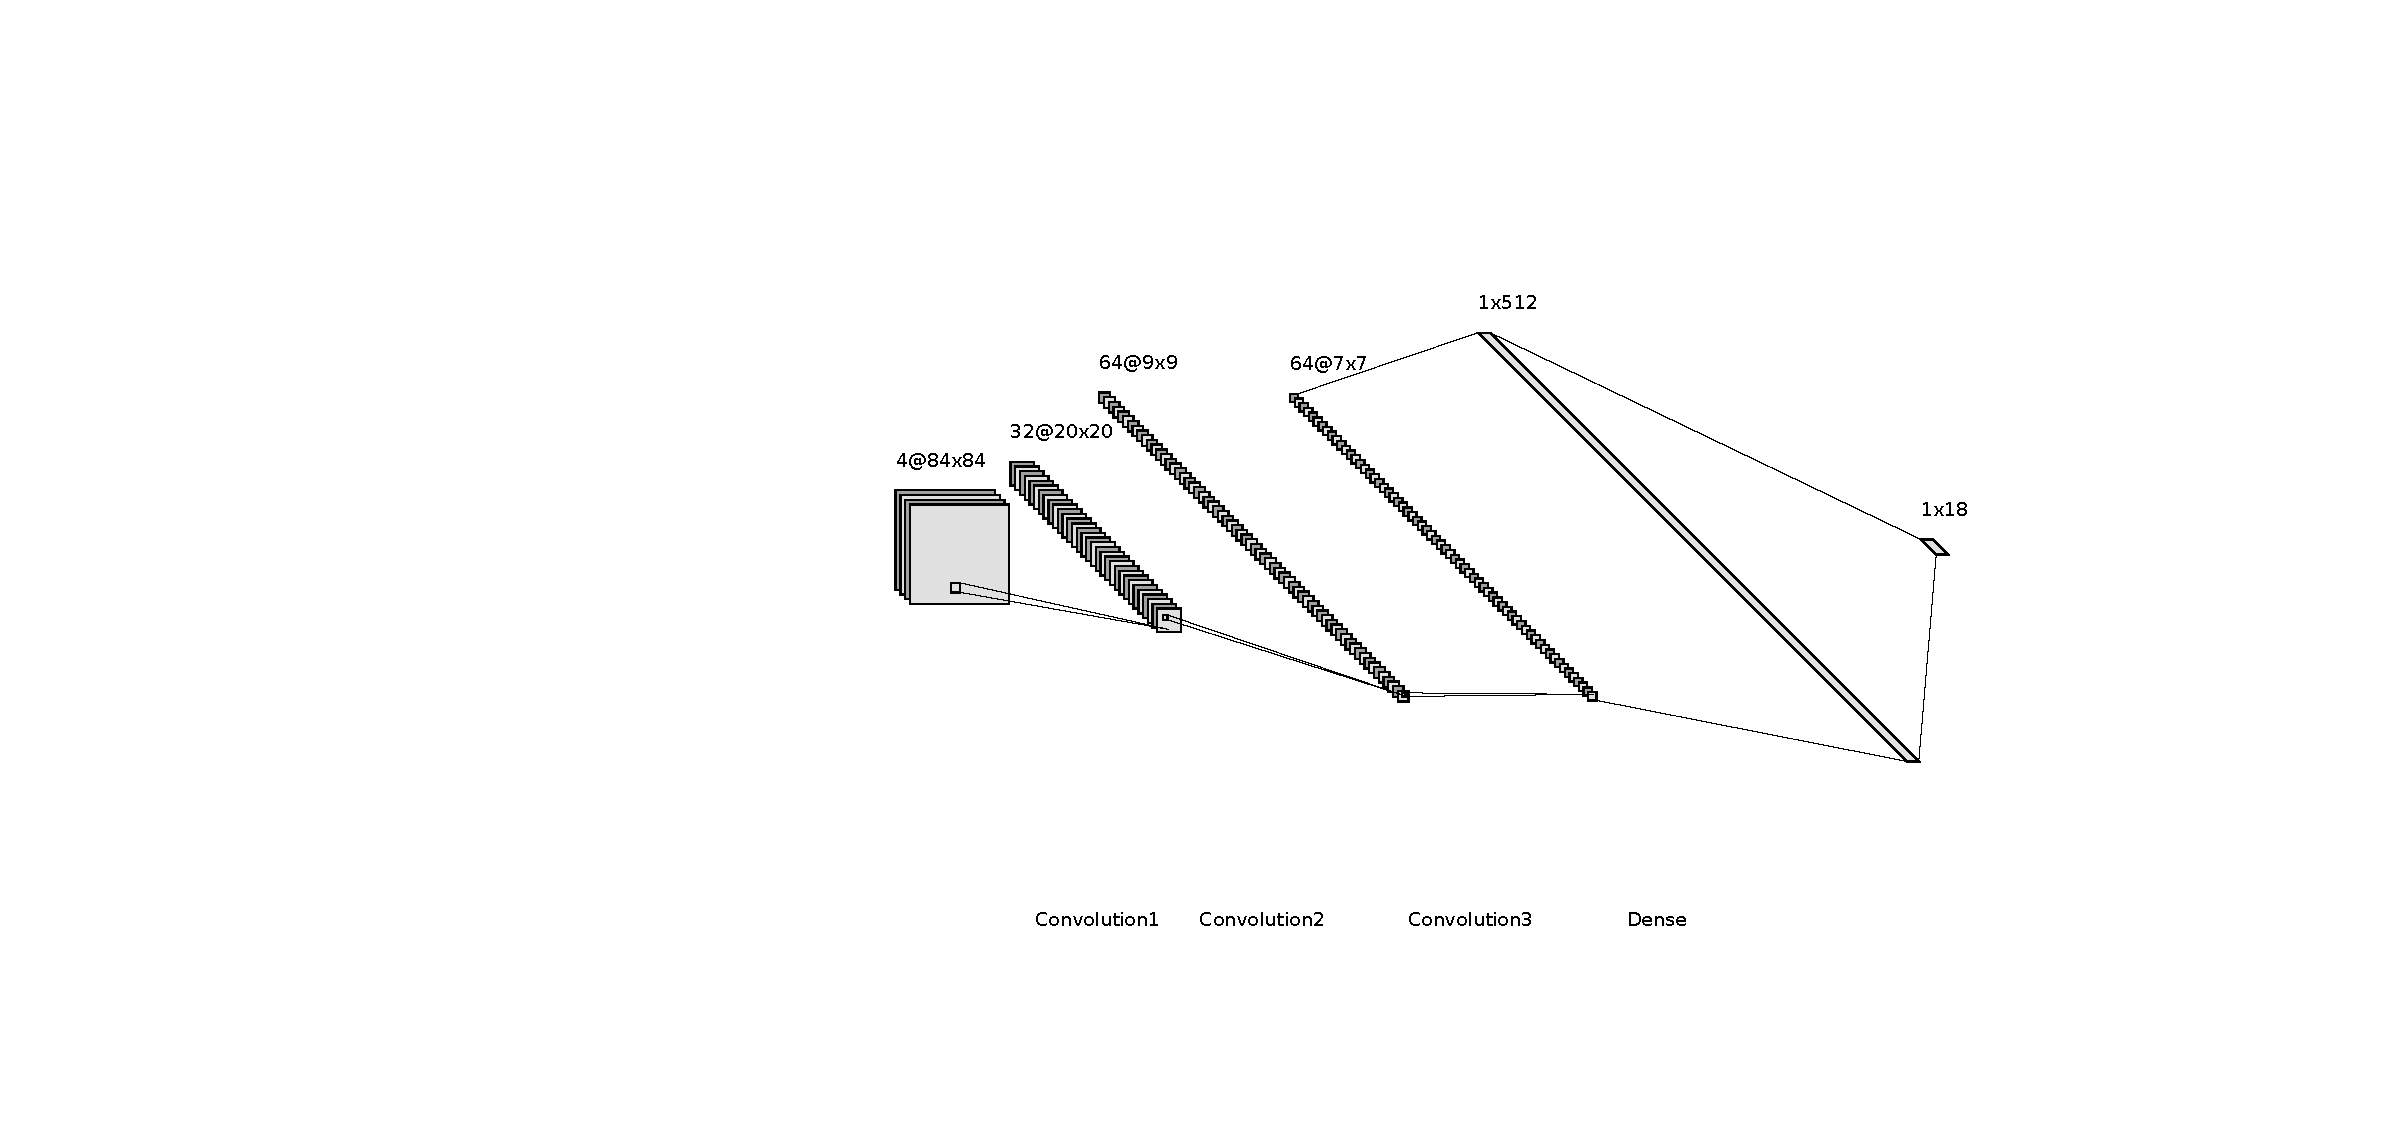
\includegraphics[scale=0.6]{nn (1).pdf}
\caption{The CNN architecture in the Q-Network of RiverRaid}
\label{fig:cnn}
\end{figure}
\subsection{Hyperparameter Selection}
We mainly follow the setting as Mnih et al. \cite{DBLP:journals/nature/MnihKSRVBGRFOPB15} did. And we made little changes in order to adapt to our hardware condition.\footnote{Wish we had money for more GPUs and memories.} The complete hyperparameter settings are shown in Appendix \ref{hyper}.

\subsection{Some Important Packages and Classes}
Since we are banned to directly use some useful modules in PyTorch such as \texttt{torch.nn} and \texttt{torch.optim}, it's necessary to explain which classes we wrote and relations between these classes.

\subsubsection{PyTrace}
The foremost module is packaged in \texttt{pytrace}, which is related to the construction and the backpropagation of our neural networks. To achieve this point, we implement a simple dynamic computation graph for the sequential neural network. 

There are several vital classes in this package, most of which are named in a \texttt{pytorch}'s fashion:
\begin{itemize}
    \item \texttt{tracer}: This is the basic data structure in \texttt{pytrace}. 
    The \texttt{tracer} is inherited from \texttt{torch.Tensor}. Thanks to that, many basic arithmetic operations are not in our concern. We further overwrite some methods bounded to \texttt{torch.Tensor} to support the gradient flows on our own dynamic computation graph.
    \begin{itemize}
        \item \texttt{backward}: To start a back-propagation from the leaf of the dynamic computation graph.
        \item \texttt{tracer.Sum}: To sum all the elements in a \texttt{tracer}.
        \item \texttt{tracer.Gather}: To pick a group of elements from a \texttt{tracer}
        \item \texttt{tracer.View}: To reshape a \texttt{tracer}.For example, use it to connect the \texttt{conv-layer} and
        \texttt{fully-connect layer} in a model.
    \end{itemize}
    \item \texttt{Operator}: This is a basic class for all kinds of operators in neural networks, by extending the basic class, we mainly implement the forward and backward function with respect to the following operators we will use in our experiment:
    \begin{itemize}
        \item \texttt{Linear}: A linear operator takes the form of $f(\mathbf{x}; \mathbf{W, b}) = \mathbf{Wx+b}$ as the output. Where $\mathbf{W, b}$ are parameters.
        \item \texttt{ReLU}: An activate function takes the form of $f(x) = \max(0, x)$.
        \item \texttt{Conv2d}: The convolution layer.
        \item \texttt{MSE}: The mean square loss takes the form of $f(\hat{\mathbf{x}}; \mathbf{x}) = \|\mathbf{x} - \hat{\mathbf{x}}\|^2$.
    \end{itemize}
    
All the operators take \texttt{data batch} into consideration. Note that, unlike some auto-grad implementations that use a so-called \texttt{gradient tape} to record the gradient-flow, we record the dynamic computation graph by connecting the \texttt{Operator} (the edge of dynamic computation graph). See details in \texttt{pytrace.nn}. 
    \item \texttt{Model}: This is a meta class for constructing a neural network by stacking the modules in \texttt{Operator}. We already pre-defined a subclass called \texttt{Sequential} for fast constructing models.
    \item \texttt{Optimizer}: We implement \texttt{RMSprop} in this class, each parameter in the optimizer is a iterable object with its original value and the gradient corresponding to present time step. And we update these parameters according to \cite{hinton}.
    \item \texttt{Initialization}: We implement some initialize methods in \texttt{pytrace.init}, including \texttt{kaiming\_uniform} and \texttt{kaiming\_normal}
\end{itemize}
For more information, please check our repository in GitHub \footnote{\url{https://github.com/gusye1234/PyTrace}}, where we offer code snippets and specific libraries we used in \texttt{pytrace}.

\subsubsection{Wrapper}
For the sake of making the game environment in a simpler fashion, we designed a module called \texttt{atari\_wrapper.py} \footnote{We mainly refers to OpenAI's work in DQN: \url{https://github.com/openai/baselines}} to adapt to DQN training in the RiverRaid environment. And the main subclasses extended by \texttt{gym.Wrapper} are listed below:
\begin{itemize}
    \item \texttt{NoopResetEnv}: Sample initial states by taking random number of no-ops on reset.
    \item \texttt{FireResetEnv}: Take action on reset for environments that are fixed until firing.
    \item \texttt{WarpFrame}: Warp frames to 84x84 as done in the Nature paper and later work
    \item \texttt{EpisodicLifeEnv}: Make end-of-life equals to end-of-episode, but only reset on true game over. It helps value estimation.
    \item \texttt{ClipRewardEnv}: Binarize rewards to \{+1, 0, -1\} by its sign.
    \item \texttt{FrameStack}: Stack 4 last frames. Returns lazy array, which is much more memory efficient.
    \item \texttt{ImageToPyTorch}: Change image shape to PyTorch fashion.
\end{itemize}

\section{Results}
In this section we will report the training process of our agent and their performance in two games. 

\subsection{Training Process}
The average 100-episode reward as well as the best mean reward of LunarLander and RiverRaid, and the learning curves are shown in Figure \ref{fig: curv}. (a) and (c) shows that the agent learned how to get higher scores as time went by.

And it's interesting noting that the learning curves didn't converge in (b) (d), which is normal in RL training. We can explain this phenomenon in two aspects. Firstly, unlike supervised regression problem, the data distribution in a RL scenario is non-stable as the parameters in DQN changes. In addition, as the reward gets higher, and the average episode length gets longer, the amount of variance in the reward can also get larger, so it's challenging even to prevent the loss from increasing.

\begin{figure}[t]
\centering

\subfigure[Rewards of LunarLander]{
\begin{minipage}[t]{0.35\linewidth}
\centering
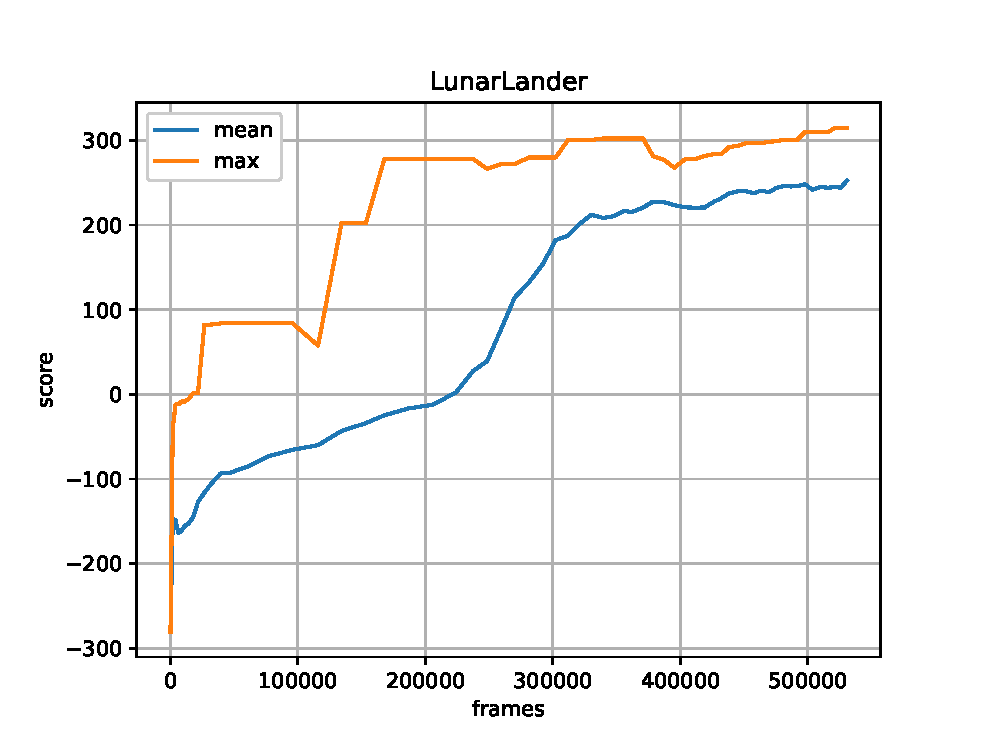
\includegraphics[width=2in]{lunarlander_score.eps}
%\caption{fig1}
\end{minipage}%
}%
\subfigure[learning curve of LunarLander]{
\begin{minipage}[t]{0.35\linewidth}
\centering
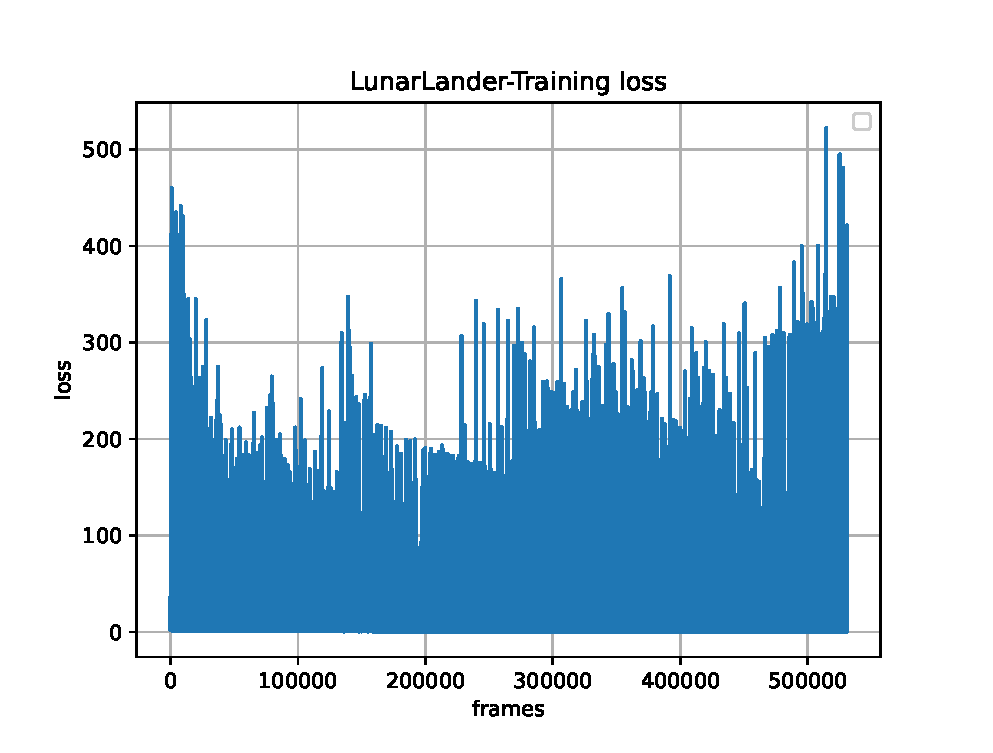
\includegraphics[width=2in]{lunarlander_loss.eps}
%\caption{fig2}
\end{minipage}%
}%
\quad
\subfigure[Rewards of RiverRaid (cliped)]{
\begin{minipage}[t]{0.35\linewidth}
\centering
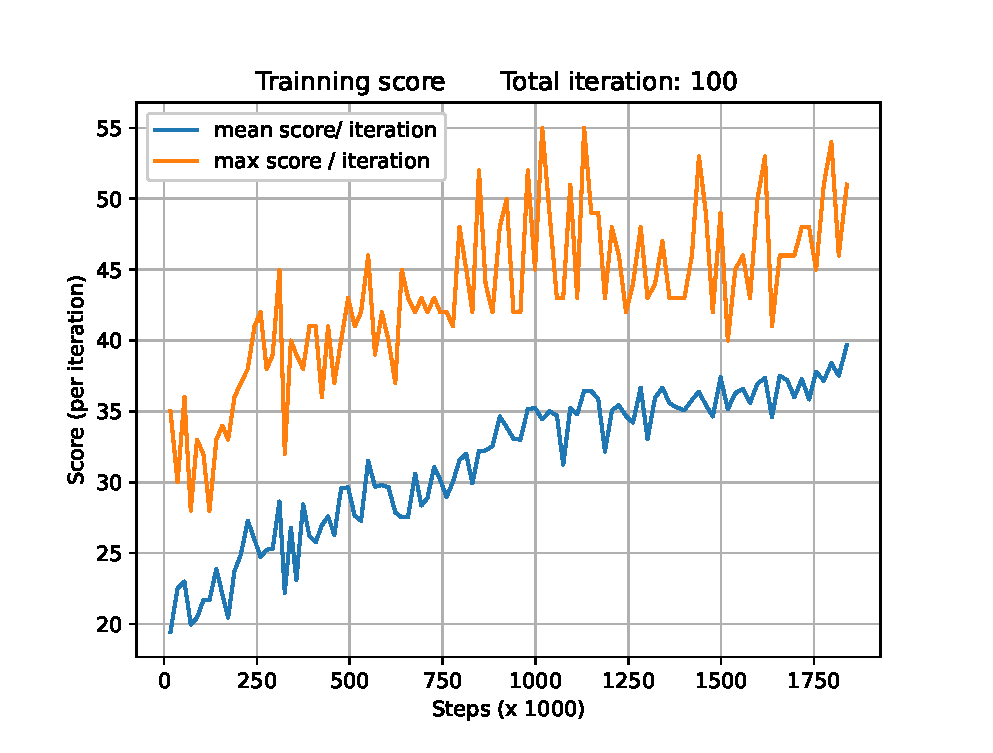
\includegraphics[width=2in]{Riverraid Score.eps}
%\caption{fig2}
\end{minipage}
}%
\subfigure[learning curve of RiverRaid ]{
\begin{minipage}[t]{0.35\linewidth}
\centering
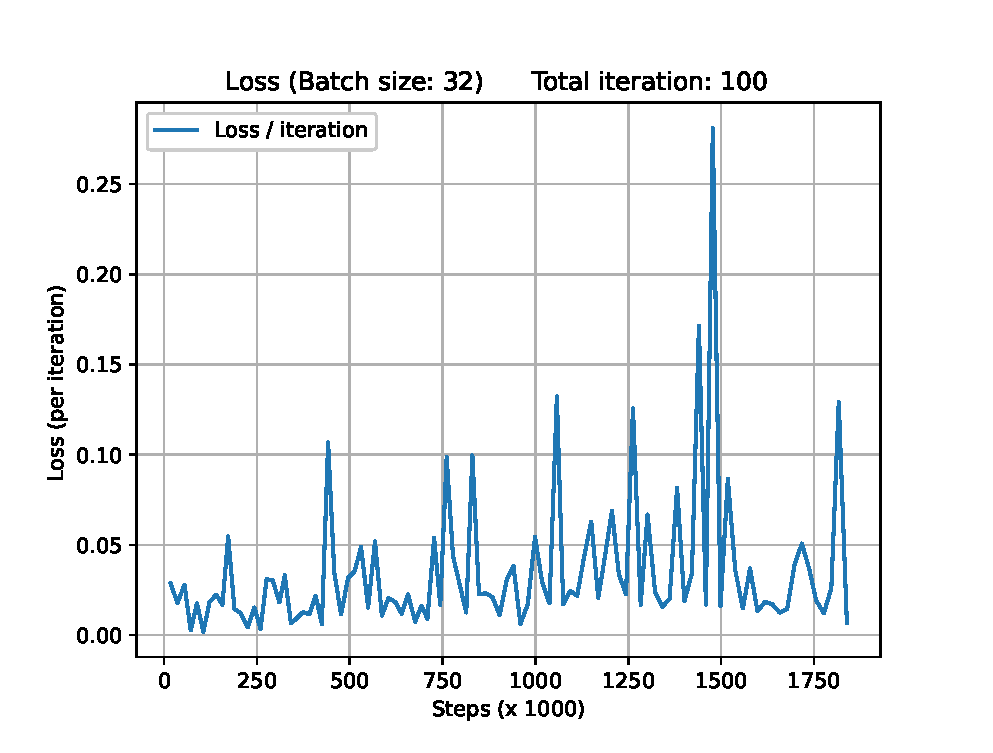
\includegraphics[width=2in]{Riverraid Loss.eps}
%\caption{fig2}
\end{minipage}
}%
\centering
\caption{\label{fig: curv}(a) and (c) shows the average 100-episode reward as well as the best mean reward of LunarLander and RiverRaid (To train the agent better, we clip the reward during training process, that is, set all the positive reward as 1, negative one as -1 and else as 0. The reason will be discussed below), respectively. (b) and (d) shows the learning curve of LunarLander and RiverRaid, respectively.}
\end{figure}

\subsection{Performances}
To evaluate the performance of our trained agent, we test our agent performance compared to random policies, the results are the averages over 100 episodes, are shown in Table \ref{result}, which shows that our agent have learned to play these games through DQN training process.
\begin{table}[!htp]
    \caption{\label{result}The Comparison Between Random Policies and Trained DQN Agents}
    \centering
    \begin{tabular}{p{100pt}p{100pt}p{50pt}}
    \toprule
    Game & Random & DQN\\
    \midrule
    LunarLander & -185 & 239\\
    RiverRaid & 1228 & 5254\\ 
    \bottomrule
    \end{tabular}
\end{table}

By watching the trained agent playing, we find that in LunarLander, the agent firstly crush itself on the lunar, which leads to a very negative reward. However, after training, the agent learned to balance itself while floating in the air, and further learned to land softly by puffing gases.

And in RiverRaid, the agent firstly behaved like a chicken with its head cut off: it was killed immediately neither by the enemies nor by crushing on the edge. While after training, we find the agent learned to shoot the enemies and to avoid the edges, which gives the agent more opportunities to earn more rewards.



\subsection{Discussion of different model in RiverRaid}
Since it's a common problem that we need to use a lot of computing resources and time to train the agent in RiverRaid. So in this part we compare several combination of different methods for training and try to find a more efficient one. All learning curve plots show scores and loss were generated using the same code base, with the same random seed initialization and the same hyperparameters as well as training iteration.The hyperparameters of these training process are listed in \textbf{Appendices} \ref{hyper}, and each agent were trained for 162 iteration (about 2.5M frames).

Figure \ref{fig:diff-dqn} shows that the "Clip + Soft" model achieves the best score in the test of 100 episodes of RiverRaid-v0. And the "Hard update" model has the worst performance. From the figure of training score of each model, it's natural to make these assumptions.

\begin{itemize}
    \item Although the game RiverRaid does not have any negative reward and positive reward range from 30 to 500 which may make it harder for agent to distinguish different enemies if we clip reward in the training process, the clip reward one perform much better than the one without. This might result from clipping reward increases the training stability since the loss is always in $ [0,1] $, while the unclipped one’s loss may be huge, causing a lot change in every update process.
    \item We can also compare the soft update one to the hard update one to conclude that the soft update does increase the stability and the performance of the agent. Both the soft and hard updates of the target network ensures that the targets of the Q-learning does not change abruptly as we are updating the Q-network weights thus helps in stabilizing the learning,  but the soft update makes the training curve more smooth than the hard update one (see in \textbf{Appendices} \ref{Models}) and thus leads better result in test.

    \item It’s still unclear now why the double DQN doesn't perform well in the training and test. Since double DQN can alleviate the “overestimates” problem and averagely perform better than DQN in \cite{hasselt2015deep}. We guess one reason might be the hyperparameters’ setting, the other might come from short training time (see in \textbf{Appendices} \ref{Models}).
\end{itemize}

\begin{figure}[t]
\centering
\subfigure[Test score of different methods]{
\begin{minipage}[t]{0.50\linewidth}
\centering
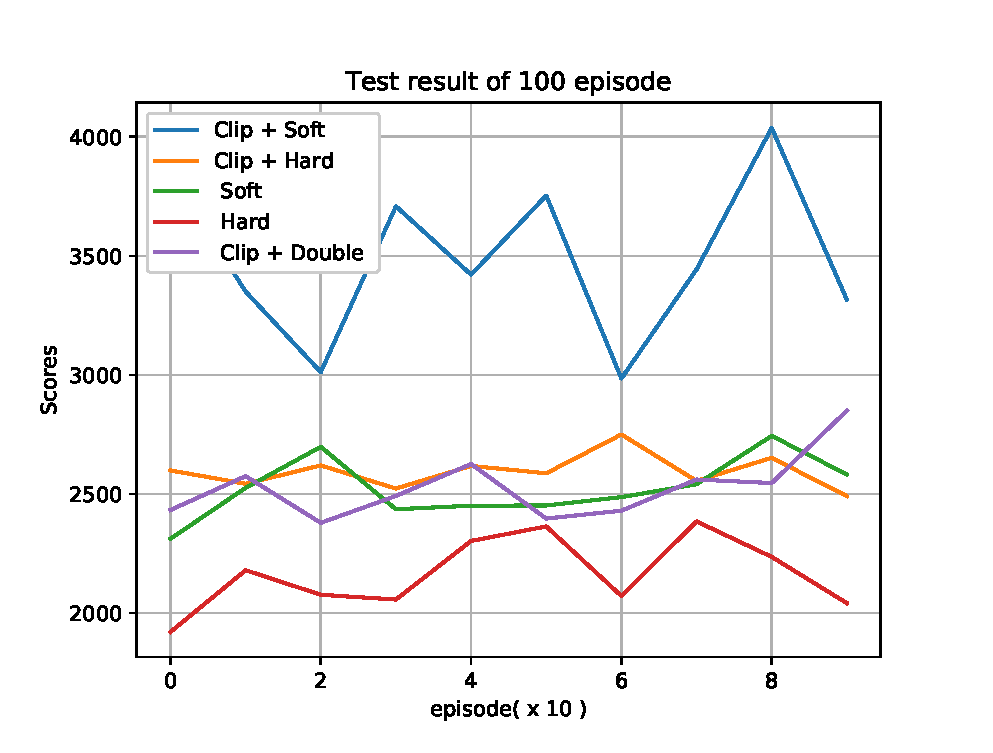
\includegraphics[width=2.5in]{pic/compare.eps}
%\caption{fig1}
\end{minipage}%
}%
\subfigure[Test score of best trained agent]{
\begin{minipage}[t]{0.50\linewidth}
\centering
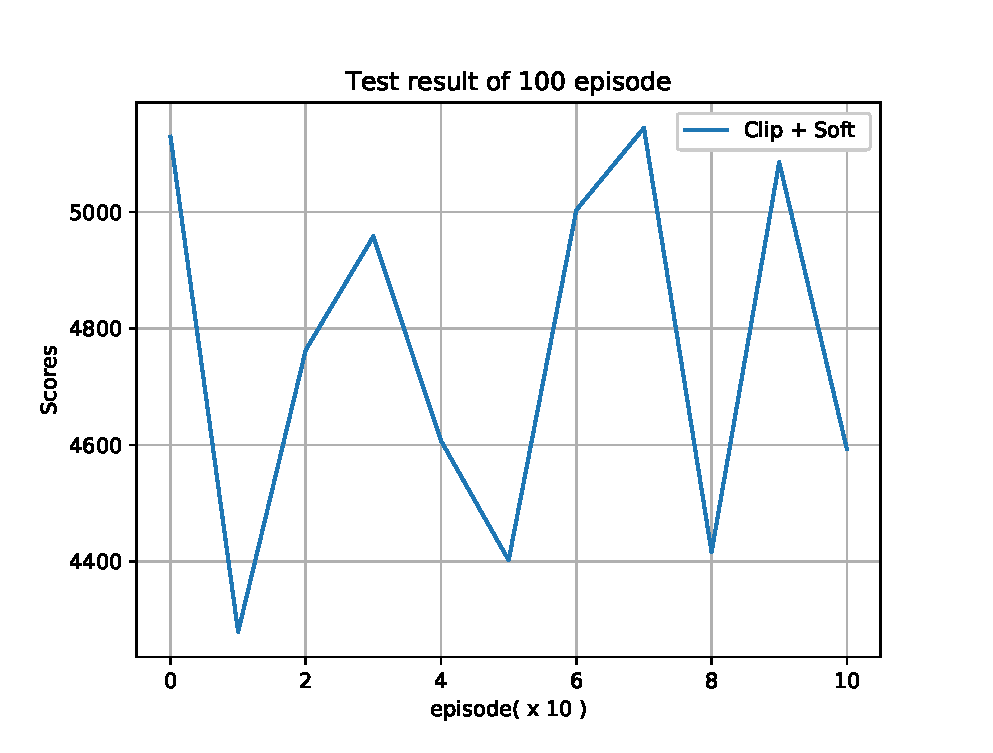
\includegraphics[width=2.5in]{RiverraidtestScore.eps}
%\caption{fig2}
\end{minipage}%
}%
\quad

\caption{\label{fig:diff-dqn}\textbf{(a)} : We compared the performance of different agent which trained under the exactly same condition except the training methods. Each agent was tested for 100 episodes and we plotted the mean score of every 10 episodes. \textbf{  (b)} : The best trained agent performance over 100 episodes}
\end{figure}

\section{Conclusions}
In this project, we first reproduce the DQN model as \cite{DBLP:journals/nature/MnihKSRVBGRFOPB15} in PyTorch to play LunarLander game, and we achieve a quite satisfying score. Then further we trained different DQN-based models in RiverRaid game, and the agent learned how to play the game better. Finally, as we are sure that our model works, we started to code our own autograd module, neural network module and other useful modules. Especially the \texttt{pytrace} module, which we think is the most highlighted part of our project.

However, there are still some points that we are able to improve further. Our performance in RiverRaid has not achieve the performance in the original papers, which we consider as a question of tuning hyperparameters. Unfortunately, restricted by the computational resources and lacked of experiences, our chosen hyperparameters have not yet reveal the maximum power of our models. 

\newpage
\appendixpage
\addappheadtotoc
\begin{appendices}
\section{Hyperparameter Settings}\label{hyper}
In Lunarlander, we set the hyper-parameters as follows
\begin{table}[H]
    \caption{\label{tab:lunar-hyper}Hyperparameters of LunarLander}
    \centering
    \begin{tabular}{cc}
    \toprule
    Hyperparameter & Value\\
    \midrule
     minibatch size & 64\\
     replay memory size & 10000\\
     replay start size & 50000\\
     main-target exchange factor $\tau$ & 0.001\\
     discount factor $\gamma$ & 0.99\\
     learning rate $\alpha$ & 0.0005\\
     gradient momentum & 0.99\\
     initial exploration & 1.0\\
     final exploration & 0.01\\
     final exploration frame & 920\\
     max frame $T_{\mathrm{max}}$ & 1000\\
    \bottomrule
    \end{tabular}
\end{table}

In RiverRaid, we set the hyper-parameters as follows
\begin{table}[H]
    \caption{\label{tab:river-hyper}Hyperparameters of RiverRaid}
    \centering
    \begin{tabular}{cc}
    \toprule
    Hyperparameter & Value\\
    \midrule
     minibatch size & 32\\
     replay memory size & 1000000\\
     replay start size & 50000\\
     main-target exchange factor $\tau$ & 0.002\\
     discount factor $\gamma$ & 0.99\\
     learning rate $\alpha$ & $6.25 \times 10^{-5}$\\
     gradient momentum & 0.95\\
     initial exploration & 1\\
     final exploration & 0.1\\
     final exploration frame & 1000000\\
     
    \bottomrule
    \end{tabular}
\end{table}

\newpage
\section{Training curve of different model}\label{Models}
We tried several combinations between models and whether clip the reward or not, the training process of these combinations are shown in Figure \ref{fig: diff-model}.

\begin{figure}[h]
\centering

\subfigure[Clip + Soft]{
\begin{minipage}[t]{0.18\linewidth}
\centering
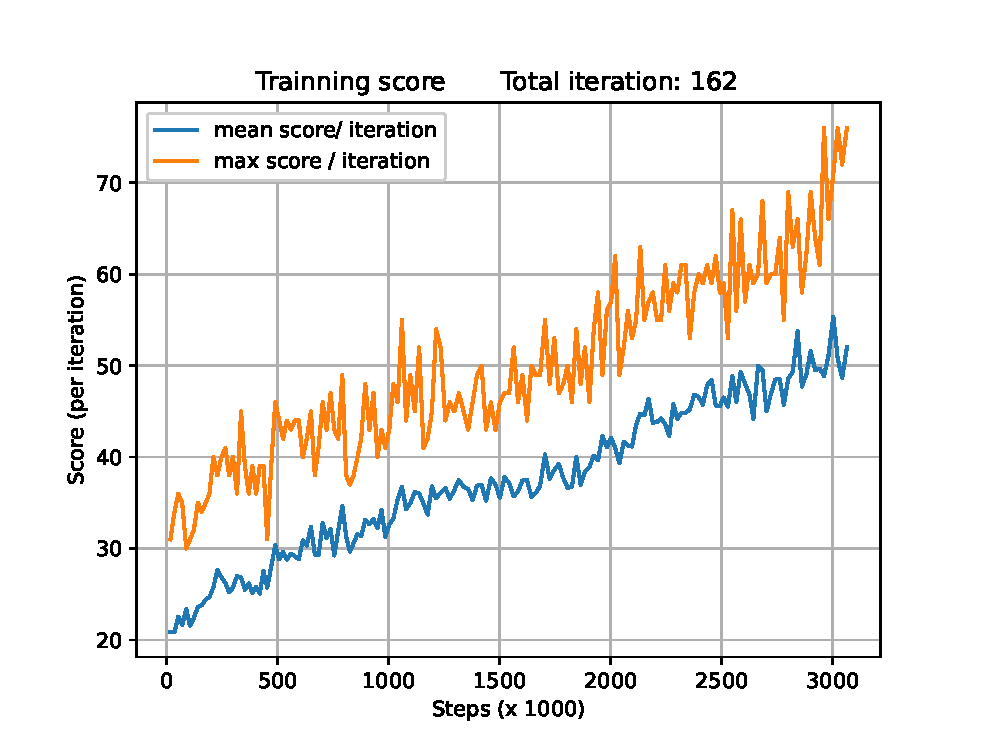
\includegraphics[width=1.2in]{Clip_Soft.eps}
%\caption{fig1}
\end{minipage}%
}%
\subfigure[Clip + Hard]{
\begin{minipage}[t]{0.18\linewidth}
\centering
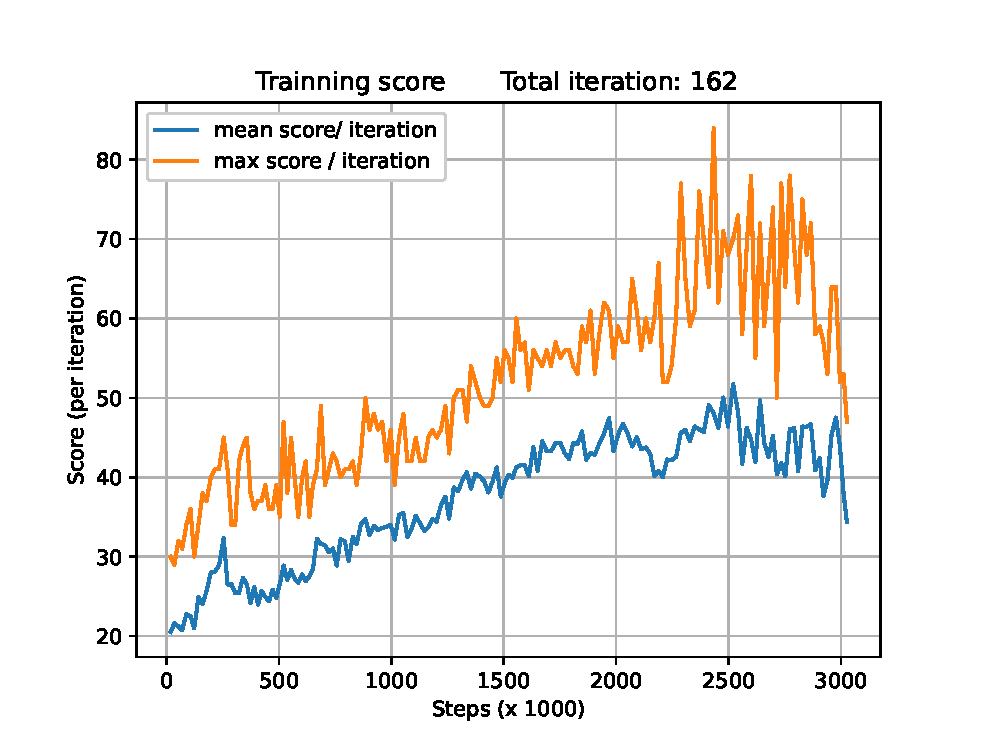
\includegraphics[width=1.2in]{Clip_Hard.eps}
%\caption{fig2}
\end{minipage}%
}%
\quad
\subfigure[Normal + Soft]{
\begin{minipage}[t]{0.18\linewidth}
\centering
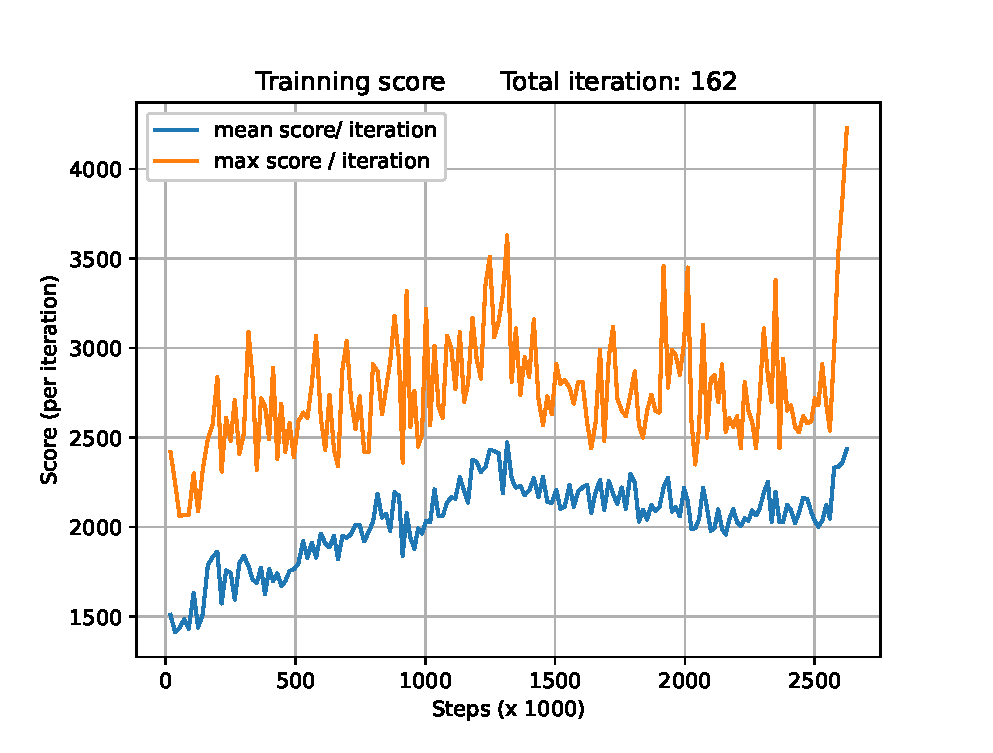
\includegraphics[width=1.2in]{Normal_Soft.eps}
%\caption{fig2}
\end{minipage}
}%
\subfigure[Normal + Hard]{
\begin{minipage}[t]{0.18\linewidth}
\centering
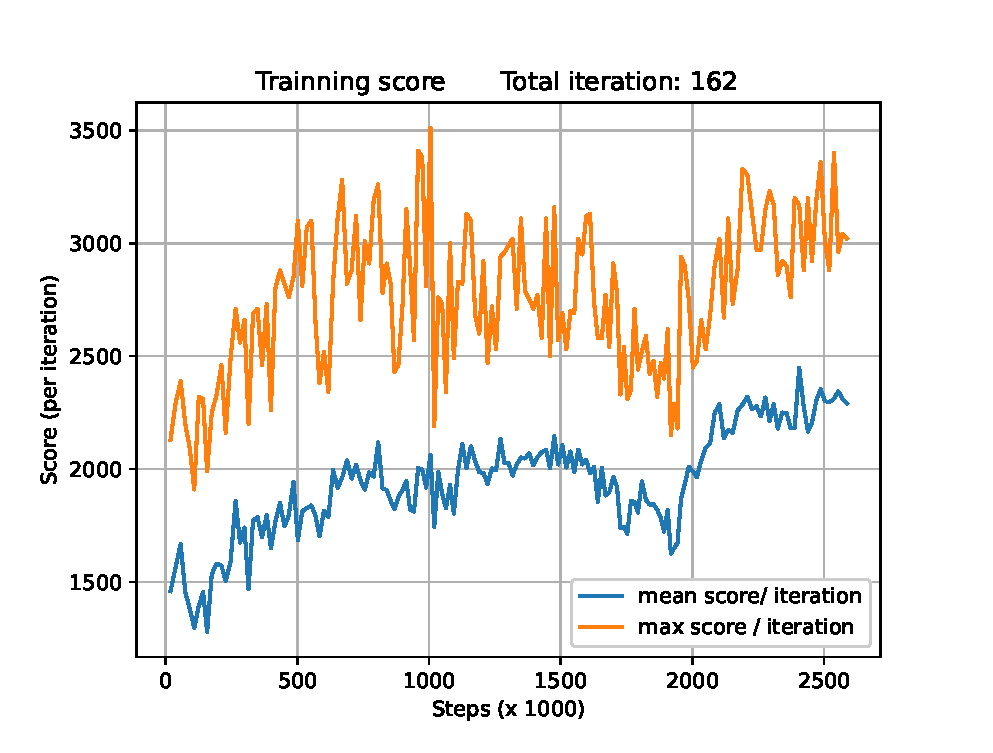
\includegraphics[width=1.2in]{Normal_Hard.eps}
%\caption{fig2}
\end{minipage}
}%
\subfigure[Clip + Double]{
\begin{minipage}[t]{0.18\linewidth}
\centering
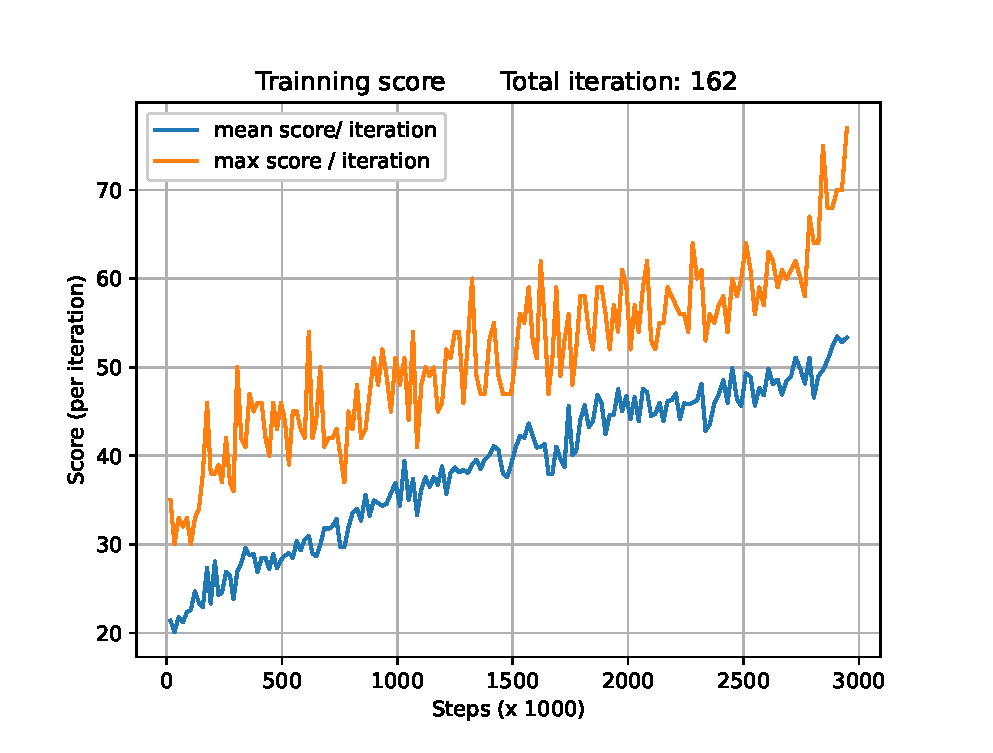
\includegraphics[width=1.2in]{Clip_Double.eps}
%\caption{fig2}
\end{minipage}
}%
\centering
\caption{\label{fig: diff-model}The training process of different combinations}
\end{figure}

\section{Statement of Individual Contribution}
We think all of us have the same contribution to the project, that is, $33\%$ for everyone. Before June 9, we all personally investigate some state-of-the-art DQN models and reproduced it on PyTorch. And then, Jianbai Ye's contribution mainly on coding \texttt{pytrace} framework and tuning the parameters of LunarLander. Xiaolong Luo's contribution mainly on tuning the parameters of RiverRaid. Shuxian Bi's contribution mainly on writting the technical report.


\end{appendices}

\newpage
\bibliographystyle{plain}  
\bibliography{ref}
\end{document}